\section{The Solenoid and the Steel Return Yoke}
\label{sec:solenoid}

The Compact Muon \emph{Solenoid} sports one of the world's most energetic solenoids which is paramount to the success of CMS.
Particles that exit the HCAL (Sec.~\ref{sec:hcal}) arrive at the cylindrical magnet which is 12.5\meter in length, has a bore diameter of 6\meter (6.3\meter when cold), and generates a uniform 3.8\tesla magnetic field parallel to the beam line.
To produce such a large and uniform magnetic field inside the approximately 360$\meter^3$ volume (Fig.~\ref{fig:cms_magnetic_field}), an 18\,000 amp current travels through the 4-layer, superconducting, NbTi coils.
This magnetic field stores a massive 2.6\GJ of energy---approximately the kinetic energy of an Airbus A320 in flight---and is 100\,000 times stronger than Earth's magnetic field, as measured on the surface.
The magnet has such a large stored-energy-to-cold-mass ratio (11.6\KJ/\Kgns) that it experiences a physical deformation of 0.15\% while being energized.
%%%%%%%%%%%%%%%%%%%%
\begin{multiFigure}
    \centering
    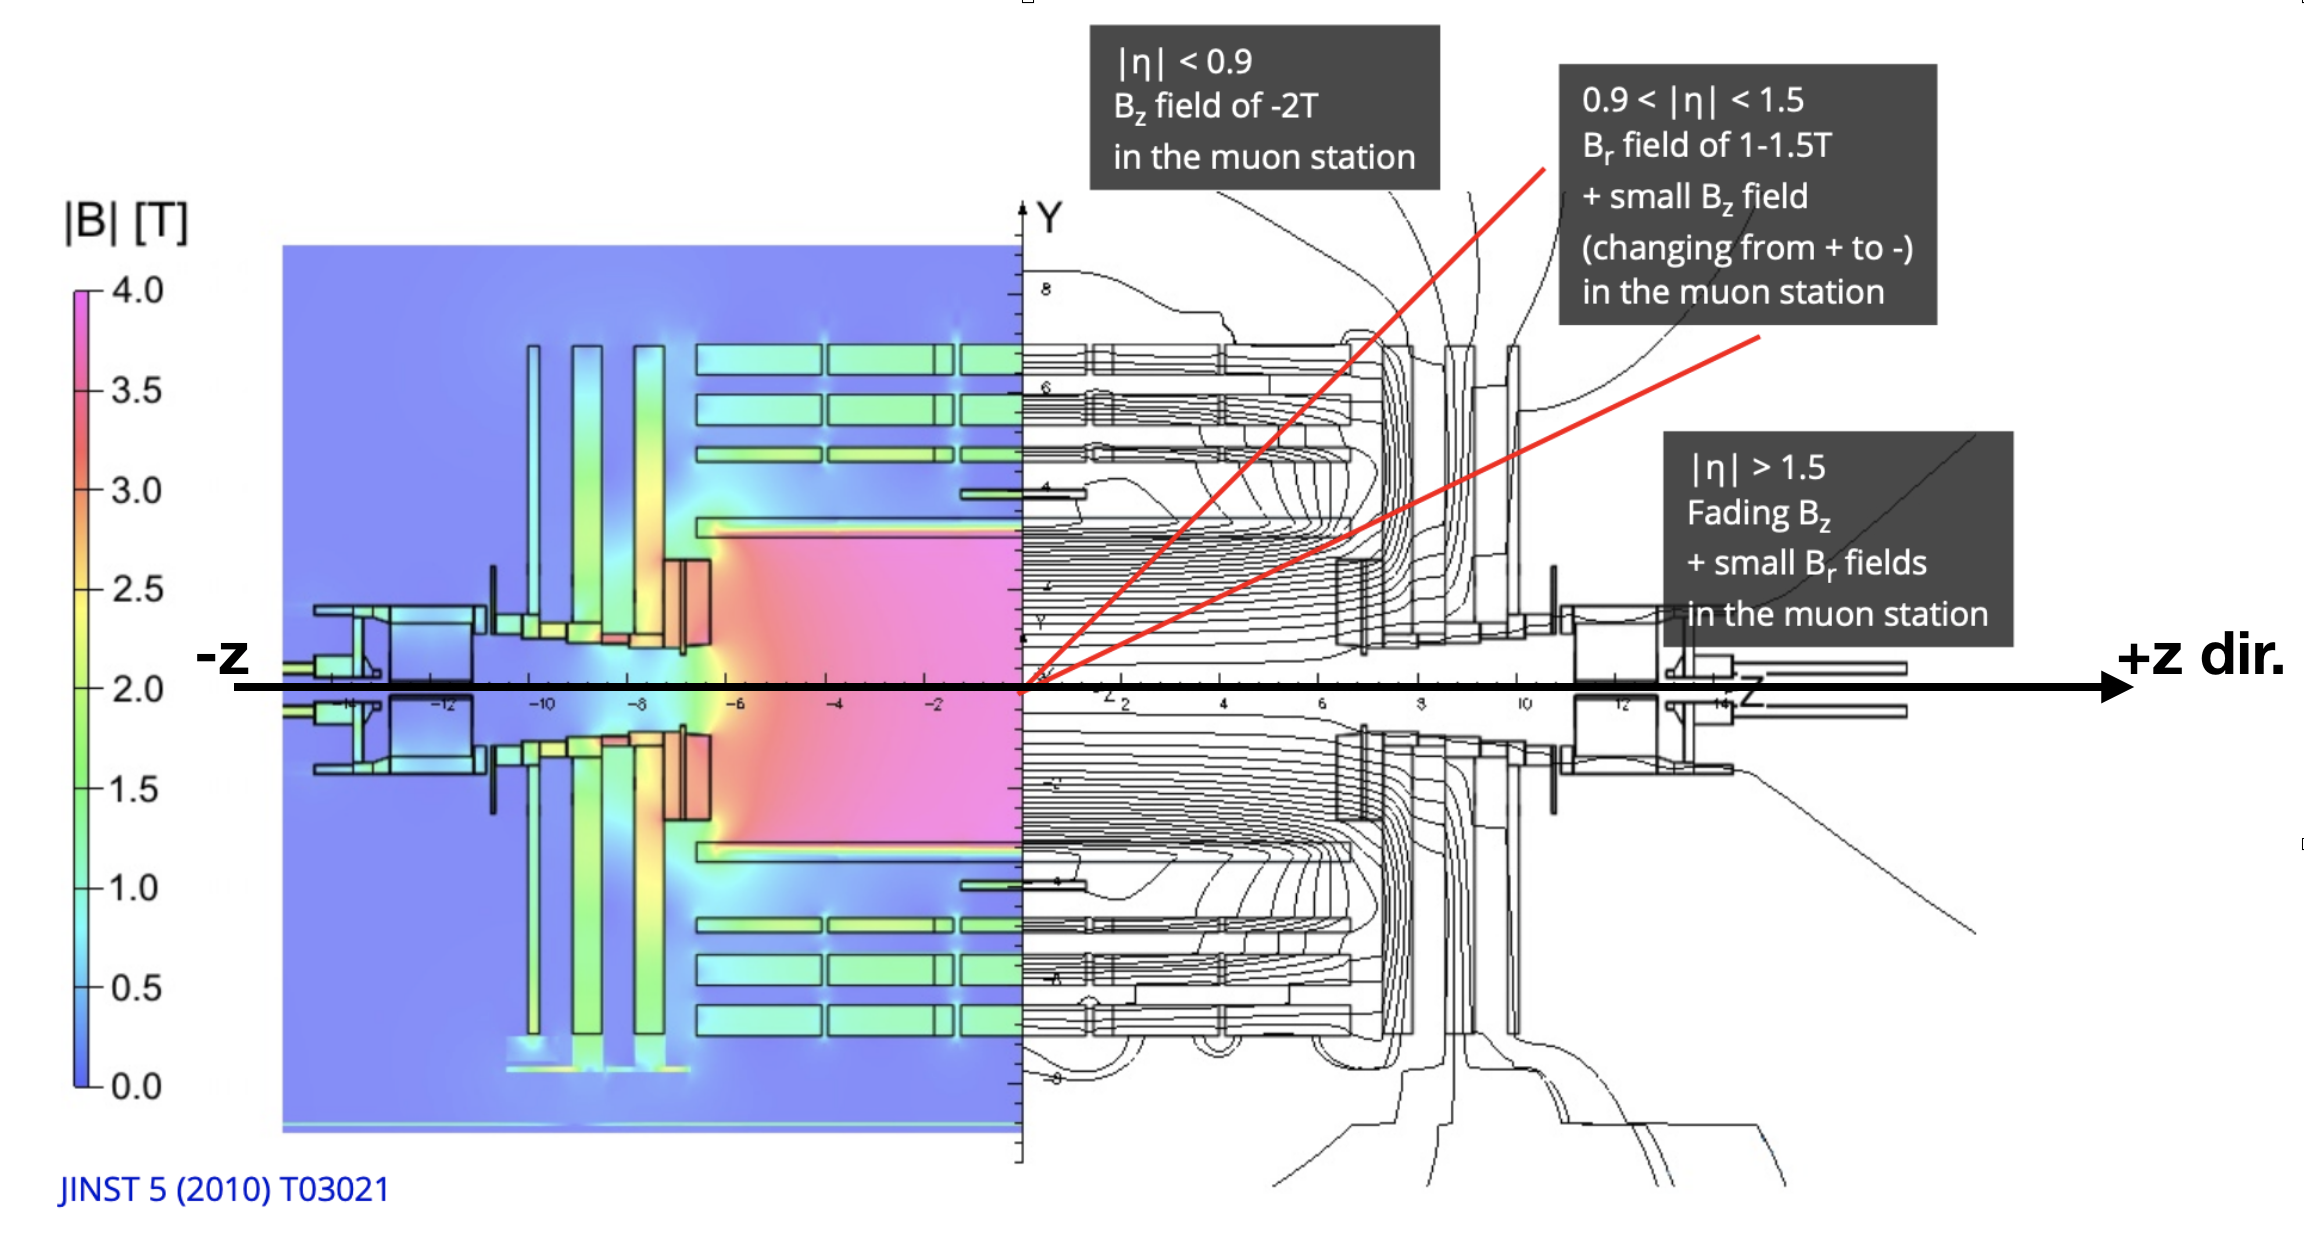
\includegraphics[width=\textwidth]{figures/cms/solenoid/CMS_longitudinal_view_magnetic_field.png}
    \captionof{figure}
        [Longitudinal cross section of CMS showing magnetic field line strength]
        {A longitudinal cross section of CMS showing the values of the magnetic field over the volume of CMS. 
        The magnetic field reaches its uniform and maximum value of 3.8\tesla in the center of the detector.
        Each magnetic field line represents a magnetic flux increment of 6\,Wb.
        Figure taken from~\cite{mag_field_lines} and modified to contain text boxes and red lines separating regions of \abseta.
        }
    \label{fig:cms_magnetic_field}
\end{multiFigure}
%%%%%%%%%%%%%%%%%%%%

As charged particles travel through any magnetic field, they experience a magnetic (Lorentz) force perpendicular to their direction of travel.
The Lorentz force $\left( \vec{F}_B \right)$ exerted on a particle with charge $q$ depends on the particle's velocity $\left( \vec{v} \right)$ and the magnetic field $\left( \vec{B} \right)$ via the cross product
\begin{equation*}
    \vec{F}_B = q \vec{v} \times \vec{B}.
\end{equation*}
Since the force is necessarily perpendicular to the velocity, the resulting trajectory is helical.
Projecting the helix on the $x$-$y$ plane (since the magnetic field points in the $+z$ direction) allows the particle tracks to typically be separated from one another.
Each track has a corresponding radius of curvature $\left( R \right)$ which relates to its transverse momentum $\left( \pt \right)$ through
\begin{equation*}
    \pt = qBR.
\end{equation*}
The relative change in \pt (\ie the \emph{momentum resolution}) is given by
\begin{equation}
    \frac{\delta \pt}{\pt} \propto \frac{\pt}{BL^2}.
\end{equation}

\textbf{Steel Return Yoke:} 
Most of the mass of CMS comes from the \emph{steel return yoke} which helps to redirect the magnetic field back on itself. 
The yoke system constitutes 10\,000 tonnes, which is 89\% of the total mass of CMS.
It is comprised of 5 wheels and 2 endcaps.
